% Options for packages loaded elsewhere
\PassOptionsToPackage{unicode}{hyperref}
\PassOptionsToPackage{hyphens}{url}
%
\documentclass[
]{article}
\usepackage{amsmath,amssymb}
\usepackage{lmodern}
\usepackage{iftex}
\ifPDFTeX
  \usepackage[T1]{fontenc}
  \usepackage[utf8]{inputenc}
  \usepackage{textcomp} % provide euro and other symbols
\else % if luatex or xetex
  \usepackage{unicode-math}
  \defaultfontfeatures{Scale=MatchLowercase}
  \defaultfontfeatures[\rmfamily]{Ligatures=TeX,Scale=1}
\fi
% Use upquote if available, for straight quotes in verbatim environments
\IfFileExists{upquote.sty}{\usepackage{upquote}}{}
\IfFileExists{microtype.sty}{% use microtype if available
  \usepackage[]{microtype}
  \UseMicrotypeSet[protrusion]{basicmath} % disable protrusion for tt fonts
}{}
\makeatletter
\@ifundefined{KOMAClassName}{% if non-KOMA class
  \IfFileExists{parskip.sty}{%
    \usepackage{parskip}
  }{% else
    \setlength{\parindent}{0pt}
    \setlength{\parskip}{6pt plus 2pt minus 1pt}}
}{% if KOMA class
  \KOMAoptions{parskip=half}}
\makeatother
\usepackage{xcolor}
\IfFileExists{xurl.sty}{\usepackage{xurl}}{} % add URL line breaks if available
\IfFileExists{bookmark.sty}{\usepackage{bookmark}}{\usepackage{hyperref}}
\hypersetup{
  pdftitle={Review of The Interaction of Wildfire Risk Mitigation Policies in the Presence of Spatial Externalities and Heterogeneous Landowners, Al Abri, Goran, 2019},
  hidelinks,
  pdfcreator={LaTeX via pandoc}}
\urlstyle{same} % disable monospaced font for URLs
\usepackage[margin=1in]{geometry}
\usepackage{color}
\usepackage{fancyvrb}
\newcommand{\VerbBar}{|}
\newcommand{\VERB}{\Verb[commandchars=\\\{\}]}
\DefineVerbatimEnvironment{Highlighting}{Verbatim}{commandchars=\\\{\}}
% Add ',fontsize=\small' for more characters per line
\usepackage{framed}
\definecolor{shadecolor}{RGB}{248,248,248}
\newenvironment{Shaded}{\begin{snugshade}}{\end{snugshade}}
\newcommand{\AlertTok}[1]{\textcolor[rgb]{0.94,0.16,0.16}{#1}}
\newcommand{\AnnotationTok}[1]{\textcolor[rgb]{0.56,0.35,0.01}{\textbf{\textit{#1}}}}
\newcommand{\AttributeTok}[1]{\textcolor[rgb]{0.77,0.63,0.00}{#1}}
\newcommand{\BaseNTok}[1]{\textcolor[rgb]{0.00,0.00,0.81}{#1}}
\newcommand{\BuiltInTok}[1]{#1}
\newcommand{\CharTok}[1]{\textcolor[rgb]{0.31,0.60,0.02}{#1}}
\newcommand{\CommentTok}[1]{\textcolor[rgb]{0.56,0.35,0.01}{\textit{#1}}}
\newcommand{\CommentVarTok}[1]{\textcolor[rgb]{0.56,0.35,0.01}{\textbf{\textit{#1}}}}
\newcommand{\ConstantTok}[1]{\textcolor[rgb]{0.00,0.00,0.00}{#1}}
\newcommand{\ControlFlowTok}[1]{\textcolor[rgb]{0.13,0.29,0.53}{\textbf{#1}}}
\newcommand{\DataTypeTok}[1]{\textcolor[rgb]{0.13,0.29,0.53}{#1}}
\newcommand{\DecValTok}[1]{\textcolor[rgb]{0.00,0.00,0.81}{#1}}
\newcommand{\DocumentationTok}[1]{\textcolor[rgb]{0.56,0.35,0.01}{\textbf{\textit{#1}}}}
\newcommand{\ErrorTok}[1]{\textcolor[rgb]{0.64,0.00,0.00}{\textbf{#1}}}
\newcommand{\ExtensionTok}[1]{#1}
\newcommand{\FloatTok}[1]{\textcolor[rgb]{0.00,0.00,0.81}{#1}}
\newcommand{\FunctionTok}[1]{\textcolor[rgb]{0.00,0.00,0.00}{#1}}
\newcommand{\ImportTok}[1]{#1}
\newcommand{\InformationTok}[1]{\textcolor[rgb]{0.56,0.35,0.01}{\textbf{\textit{#1}}}}
\newcommand{\KeywordTok}[1]{\textcolor[rgb]{0.13,0.29,0.53}{\textbf{#1}}}
\newcommand{\NormalTok}[1]{#1}
\newcommand{\OperatorTok}[1]{\textcolor[rgb]{0.81,0.36,0.00}{\textbf{#1}}}
\newcommand{\OtherTok}[1]{\textcolor[rgb]{0.56,0.35,0.01}{#1}}
\newcommand{\PreprocessorTok}[1]{\textcolor[rgb]{0.56,0.35,0.01}{\textit{#1}}}
\newcommand{\RegionMarkerTok}[1]{#1}
\newcommand{\SpecialCharTok}[1]{\textcolor[rgb]{0.00,0.00,0.00}{#1}}
\newcommand{\SpecialStringTok}[1]{\textcolor[rgb]{0.31,0.60,0.02}{#1}}
\newcommand{\StringTok}[1]{\textcolor[rgb]{0.31,0.60,0.02}{#1}}
\newcommand{\VariableTok}[1]{\textcolor[rgb]{0.00,0.00,0.00}{#1}}
\newcommand{\VerbatimStringTok}[1]{\textcolor[rgb]{0.31,0.60,0.02}{#1}}
\newcommand{\WarningTok}[1]{\textcolor[rgb]{0.56,0.35,0.01}{\textbf{\textit{#1}}}}
\usepackage{graphicx}
\makeatletter
\def\maxwidth{\ifdim\Gin@nat@width>\linewidth\linewidth\else\Gin@nat@width\fi}
\def\maxheight{\ifdim\Gin@nat@height>\textheight\textheight\else\Gin@nat@height\fi}
\makeatother
% Scale images if necessary, so that they will not overflow the page
% margins by default, and it is still possible to overwrite the defaults
% using explicit options in \includegraphics[width, height, ...]{}
\setkeys{Gin}{width=\maxwidth,height=\maxheight,keepaspectratio}
% Set default figure placement to htbp
\makeatletter
\def\fps@figure{htbp}
\makeatother
\setlength{\emergencystretch}{3em} % prevent overfull lines
\providecommand{\tightlist}{%
  \setlength{\itemsep}{0pt}\setlength{\parskip}{0pt}}
\setcounter{secnumdepth}{-\maxdimen} % remove section numbering
\ifLuaTeX
  \usepackage{selnolig}  % disable illegal ligatures
\fi

\title{Review of \emph{The Interaction of Wildfire Risk Mitigation
Policies in the Presence of Spatial Externalities and Heterogeneous
Landowners}, Al Abri, Goran, 2019}
\author{}
\date{\vspace{-2.5em}2022-07-27}

\begin{document}
\maketitle

\hypertarget{contribution}{%
\subsection{Contribution}\label{contribution}}

This paper investigates the game interaction surrounding wildfire
prevention in a landscape with different owners. In a dynamic model of
vegetation growth, landowners choose how much forest to cut down to
prevent wildfires. Considering that wildfire ignition risk, spread and
damage are dependent on the fuel stock, the authors investigate the
implications of different beliefs and information sets. In this setting,
landowners may operate based on misconceptions of the probabilities of
wildfires or their damages. The authors investigate how these beliefs
may lead to socially inefficient outcomes.

\hypertarget{my-comments-feelings-questions}{%
\subsection{My comments, feelings,
questions}\label{my-comments-feelings-questions}}

I'm kind of disappointed by the absence of spatial process, and the
consideration of just a forest stock. \textbackslash\textbackslash{} I'm
still kind of confused about the formulation of the fire ignition
process. Indeed, whether fire ignites in \(i\) or in \(k\) and spreads,
or in \(i\) and in \(k\) and spreads, the results are the same. There is
no intensity element.

\hypertarget{technical-issues}{%
\subsection{Technical issues}\label{technical-issues}}

While the paper raises an interesting question, it is flawed in several
respects, when it comes to its core formulation.

\hypertarget{binary-variable-for-fire-occurrence-probability-and-arrival-rate}{%
\subsubsection{Binary variable for fire occurrence, probability and
arrival
rate}\label{binary-variable-for-fire-occurrence-probability-and-arrival-rate}}

First, a random variable \(\theta_{it} \in \{0,1\}\) measures the
occurrence of fire. The arrival of fire is said to be modeled as a
Poisson distribution. However, the random variable depicted here is
binary, while Poisson processes describe a number of occurrences over a
finite period. It is therefore left to the reader how to make sense of
this formulation. Indeed, the question remains as to how \(\theta_{it}\)
maps to the Poisson process.

My interpretation is that \begin{align*}
\theta=1 &\iff X \sim P(\lambda) 
\\
&x>0
\end{align*} that is to say, fire occurs if the fire arrival variable
that follows a Poisson distribution has a realization which value is
superior to 0. Hence : \begin{align*}
    \mathcal{P}(X>0)&=1-P(X=0)\\
    &= 1- e^{-\lambda}
\end{align*} Therefore: \begin{equation}
    \mathcal{P}(\theta_{it}=1)=1-e^{-\lambda}
\end{equation}

\subsection{Concerns about the arrival rate : formulation, temporal mismatch, reliance on the forest biomass}

In eq(13) of the article, the ``arrival rate'' is defined as : \[
\lambda(\gamma, f_{jt},f_{kt})=1-e^{-\gamma\frac{k(f_{jt})+k(f_{kt})}{W}}
\] If anything, the relevant formulation here would be :
\begin{equation*}
    \lambda(\gamma, f_{jt},f_{kt})=\gamma\frac{k(f_{jt})+k(f_{kt})}{W}
\end{equation*} Which is consistent with the interpretation of an
arrival rate depending on the fuel, as it grows with the fuel.

Moreover, there seems to be a temporal mismatch. In section 2.4, the
authors write:

\begin{displayquote}
\textit{in the absence of fuel treatment of fire, forest biomass growth is given by $k(f_{it})$}
\end{displayquote}

Therefore, the biomass \textbf{ in t+1} is governed by this growth
function. It is striking that \textbf{in t}, the fire arrival rate and
hence, the probability that the parcel ignites depends on \(k(f_{it})\)

On a more conceptual note, it is unclear why the ignition rate on any
parcel depends on the total forest area. Ignition probabilities are
mostly local, depending on environmental conditions, and not necessarily
based on the amount of available fuel. Considering small neighboring
parcels, it is likely that those environmental conditions are identical.

\hypertarget{a-surprising-damage-function}{%
\subsubsection{A surprising damage
function}\label{a-surprising-damage-function}}

The formulation of the damage function is difficult to rationalize. In
equation (4), the authors posit that the damage resulting from the fire
is a \textit{decreasing} function of the standing forest. There is no
comment on this hypothesis. Later on, in table 1, which displays the
specifications of the functional forms : \begin{align*}
& D_{it}=e^{-\frac{0.1}{f_{it}}}\\
& \Rightarrow \frac{\partial D_{it}}{\partial f_{it}}=-0.1\times -\frac{1}{f_{it}}
\end{align*} Two comments are in order:

\begin{enumerate}
    \item The derivative of the damage function is clearly positive, hence contradicting equation (4):
    \begin{equation*}
        \frac{\partial D_{it}}{\partial f_{it}}=\frac{0.1}{(f_{it})^2}e^{-\frac{0.1}{f_{it}}}>0
    \end{equation*}
    \item The limits are such that : 
    \begin{align*}
        \lim_{f_{it} \to 0}D(f_{it})&=0\\
        \lim_{f_{it} \to \infty}D(f_{it})&=1
    \end{align*}
\end{enumerate}

\hypertarget{the-formulation-of-the-expected-damage}{%
\subsection{The formulation of the expected
damage}\label{the-formulation-of-the-expected-damage}}

\hypertarget{a-reformulation-of-the-papers-formula}{%
\subsubsection{A reformulation of the paper's
formula}\label{a-reformulation-of-the-papers-formula}}

Third, the formulation in equation (5) of the expected damage includes:

\begin{displayquote}
\begin{enumerate}
\item\textit{ the probability of fire occurring on parcel j and the associated damage and }
\item \textit{the probability of fire
occurring on parcel k and spreading to parcel j and the associated damage"}
\end{enumerate}
\end{displayquote}

However, the formulation of equation (5) is : \begin{equation*}
    D_{jt,total}=\theta_{jt}D(f_{jt})+\theta_{kt}\phi_{jt}(f_{kt})D(f_{jt})
\end{equation*} In this equation, except for \(\phi_{jt}\), there is no
probability. It is merely a formulation of the damage in a potential
outcome framework, without the associated probability.

A relevant expected damage function would write, in this context :
\begin{align*}
    D_{jt,total}&=D(f_{jt})\left[ \mathcal{P}(\theta_{it}=1)+\mathcal{P}(\theta_{kt}=1 \& \text{Spread from k to j}) \right]\\
    &=D(f_{jt})\left[ \mathcal{P}(\theta_{it}=1)+\mathcal{P}(\theta_{kt}=1)\times \phi_{jt}(f_{kt}) \right]\\
\end{align*}

\subsubsection{Independence and expected damage as a share}

From line 1 to line 2, the independence of ignition and spread is
required to obtain a formulation akin to that of the authors. However,
the local probability of ignition and the probability of spread both
depends on the forest stock. Therefore,
\textit{one cannot assume that the two variables are independent}.

For the sake of the argument, assuming that both ignition and spread are
independent, this would imply : \[
 D_{jt,total}=D(f_{jt})(1-e^{-\lambda})(1+\phi(f_{kt}))
\] The following graph traces the expected damage for different values
of the forest standing in the neighboring lot. It is clear that the
formulation of the damage function as a share requires additional
assumptions and that the false assumption of independence lead to
results that contradict the share formulation:

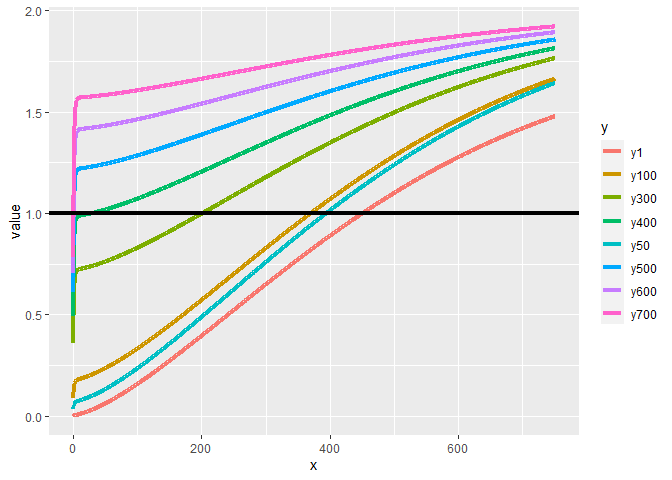
\includegraphics{Sim_files/figure-latex/unnamed-chunk-1-1.pdf}

This result is not surprising. A decomposition of the the article's
formulation of expected damage function can help explain those results :

\begin{itemize}
    \item The damage, depending on the forest stock in parcel $j$. The functional form of the damage function guarantees that $\forall f_{jt}, D(f_{jt}) \in  [0,1]$, and that it increases with $f_{jt}$
    \item The probabilities of the damage occurring : 
    \begin{itemize}
        \item The probability of ignition in site $j$ and $k$, increasing in $f_{jt}$ and $f_{kt}$, and $$\lim_{f_{kt},f_{jt}\to \infty}1-e^{-\lambda}=1$$
        \item The probability of spread which increases with $f_{kt}$ and 
        $$
        \lim_{f_{kt}\to \infty}\phi(.)=1
        $$
    \end{itemize}
\end{itemize}

The problem therefore lies in an incorrect formulation of the
\textit{burn probability} in parcel \(j\). In this setting, the
probability that parcel \(j\) does not ignite is not taken into account
when considering the spread from cell \(k\). Therefore, as both ignition
and spread probabilities increase in the stock, this formulation implies
the limit probability of fire occurrence in cell \(j\) to converge to 2
instead of 1. In the current formulation, the set of events that lead to
fire occurrence in parcel \(j\) are

\begin{itemize}
    \item Fire ignition in parcel $j$, irrespective of the other set of events (ignition and spread in parcel $k$)
    \item No ignition in parcel $j$ $\cap$ ignition in parcel $k$ $\cap$ spread from $k$ to $j$
\end{itemize}

Taking the expectation with respect to the correct formulation of the
set of events : \begin{align*}
    D_{jt,total}&=D(f_{jt})\big[ \mathcal{P}(\theta_{jt}=1)+\mathcal{P}(\theta_{jt}=0\cap \theta_{kt}=1\cap \text{Spread from k to j})\big]\\
    &=D(f_{jt})\big[ \mathcal{P}(\theta_{jt}=1)+\mathcal{P}(\theta_{jt}=0)\times \mathcal{P}( \theta_{kt}=1\cap \text{Spread from k to j})\big]\\
    &=D(f_{jt})\big[ (1-\mathcal{P}(\theta_{jt}=0))+\mathcal{P}(\theta_{jt}=0)\times \mathcal{P}( \theta_{kt}=1\cap \text{Spread from k to j})\big]\\
    &= D(f_{jt})\big[ 1+ \mathcal{P}(\theta_{jt}=0)\big(\mathcal{P}( \theta_{kt}=1\cap \text{Spread from k to j})-1\big)\big]
\end{align*} Once again, using the hypothesis of the independence of
ignition and spread for cell \(k\) : \begin{align*}
     D_{jt,total}&=D(f_{jt}))\big[ 1+ \mathcal{P}(\theta_{jt}=0)\big(\mathcal{P}( \theta_{kt}=1)\times \mathcal{P}( \text{Spread from k to j})-1\big)\big]\\
     &=D(f_{jt}))\big[ 1+ e^{-\lambda}\big((1-e^{-\lambda})\phi(f_{kt})-1\big)\big]
\end{align*} When you click the \textbf{Knit} button a document will be
generated that includes both content as well as the output of any
embedded R code chunks within the document. You can embed an R code
chunk like this:

\begin{Shaded}
\begin{Highlighting}[]
\FunctionTok{summary}\NormalTok{(cars)}
\end{Highlighting}
\end{Shaded}

\begin{verbatim}
##      speed           dist       
##  Min.   : 4.0   Min.   :  2.00  
##  1st Qu.:12.0   1st Qu.: 26.00  
##  Median :15.0   Median : 36.00  
##  Mean   :15.4   Mean   : 42.98  
##  3rd Qu.:19.0   3rd Qu.: 56.00  
##  Max.   :25.0   Max.   :120.00
\end{verbatim}

\hypertarget{including-plots}{%
\subsection{Including Plots}\label{including-plots}}

You can also embed plots, for example:

\includegraphics{Sim_files/figure-latex/pressure-1.pdf}

Note that the \texttt{echo\ =\ FALSE} parameter was added to the code
chunk to prevent printing of the R code that generated the plot.

\end{document}
